\documentclass[aspectratio=169,xcolor=dvipsnames]{beamer}
\usetheme{SimplePlus}

\usepackage{hyperref}
\usepackage{graphicx}
\usepackage{booktabs}
\usepackage{listings}
\usepackage{algorithm2e}
\usepackage{booktabs}  
\usepackage{subcaption}
\usepackage{xcolor}    
\usepackage[round]{natbib}
% \usepackage{enumitem}

\SetKwProg{Fn}{Function}{}{end}
\SetKwFunction{FRecurs}{FnRecursive}%
\SetAlgoLongEnd

\definecolor{dkgreen}{rgb}{0,0.6,0}
\definecolor{gray}{rgb}{0.5,0.5,0.5}
\definecolor{mauve}{rgb}{0.58,0,0.52}
\definecolor{codegreen}{rgb}{0,0.6,0}
\definecolor{codegray}{rgb}{0.5,0.5,0.5}
\definecolor{codepurple}{rgb}{0.58,0,0.82}
\definecolor{backcolour}{rgb}{1.00,1.00,1.00}

\lstdefinestyle{code}{language=Java,
  backgroundcolor=\color{InvisibleBlue},
  showstringspaces=false,
  columns=flexible,
  basicstyle={\ttfamily\footnotesize},
  numbers=left,
  numberstyle=\scriptsize\color{black},
  keywordstyle=\ttfamily\color{mauve},
  numbersep=5pt,
  commentstyle=\color{dkgreen},
  stringstyle=\color{mauve},
  breaklines=true,
  breakatwhitespace=false,
  tabsize=2,
  xleftmargin=1.0cm,
  framexleftmargin=1.5em,
  framesep=2pt,
  escapechar=|,
}

\newenvironment<>{varblock}[2][.9\textwidth]{%
  \setlength{\textwidth}{#1}
  \begin{actionenv}#3%
    \def\insertblocktitle{#2}%
    \par%
    \usebeamertemplate{block begin}}
  {\par%
    \usebeamertemplate{block end}%
  \end{actionenv}}

  \setbeamertemplate{footline}
  {
    \leavevmode%
    \hbox{%
    \begin{beamercolorbox}[wd=.4\paperwidth,ht=2.25ex,dp=1ex,center]{author in head/foot}%
      \usebeamerfont{author in head/foot}\insertshortauthor
    \end{beamercolorbox}%
    \begin{beamercolorbox}[wd=.6\paperwidth,ht=2.25ex,dp=1ex,center]{title in head/foot}%
      \usebeamerfont{title in head/foot}\insertshorttitle\hspace*{3em}
      \insertframenumber{} / \inserttotalframenumber\hspace*{1ex}
    \end{beamercolorbox}}%
    \vskip0pt%
  }
  \makeatletter
  \setbeamertemplate{navigation symbols}{}
  
\newcommand{\xDownarrow}[1]{%
  \ensuremath{%
    \left\Downarrow\vbox to #1{}\right.\kern-\nulldelimiterspace
  }%
}

%----------------------------------------------------------------------------------------
%	TITLE PAGE
%----------------------------------------------------------------------------------------
\title[Selective Value-Object Inlining using Hybrid Program Analysis]{Selective Value-Object Inlining using Hybrid Program Analysis}
\subtitle{M.S (By Research) Synopsis Seminar }
\titlegraphic{
  
\includegraphics[width=2.5cm]{images/iit_mandi_logo}
}
\author[A.H. Kumar] {Arjun Harikumar}
% \author[M. Thakur] {Manas Thakur}

\institute[IIT Mandi] % Your institution as it will appear on the bottom of every slide, may be shorthand to save space
{
  Guided By,

  Dr. Manas Thakur
}
% \date{\today} % Date, can be changed to a custom date


%----------------------------------------------------------------------------------------%
%	PRESENTATION SLIDES
%----------------------------------------------------------------------------------------%

\begin{document}
%------------------------- 1. START SLIDE -----------------------%
\begin{frame}
    \titlepage
\end{frame}
\logo{

\includegraphics[width=1.5cm]{images/iit_mandi_logo}
}

%------------------------- 2. OOPS SLIDE -----------------------%
\begin{frame}{Object-Oriented Paradigm}
  \begin{columns}[c] 
    \column{.42\textwidth}
    \begin{varblock}[9.5cm]{}
        \begin{itemize}
        \item OOP is one of the most widely used programming paradigm.
        \item Promotes efficient design with reusable components.
        \item Domain entities are represented as classes.
        \item Classes are instantiated using objects.
        \item All objects have identity.
        \item Identity enables mutability.
        % \item Objects change states multiple times during the course of execution.
        \end{itemize}
      \end{varblock}
      \vfill
    \column{.3\textwidth} % Right column and width
    \begin{figure}[noindent]
      
\includegraphics[scale=0.1]{images/oop-lang.pdf}
    \end{figure}
  \end{columns}
\end{frame}
%------------------------- 2. OOPS SLIDE -----------------------%

%------------------------- 3. OBJECT STRUCTURE SLIDE -----------------------%
\begin{frame}{Object Structure}
  \begin{columns}[T,onlytextwidth] 
    \column{0.45\textwidth} 
    \begin{figure}
      \lstinputlisting[style=code]{code/TransactionInfo.java}
      % \caption{Example Java classes.}
    \end{figure}
    \column{0.55\textwidth} 
    \begin{figure}
      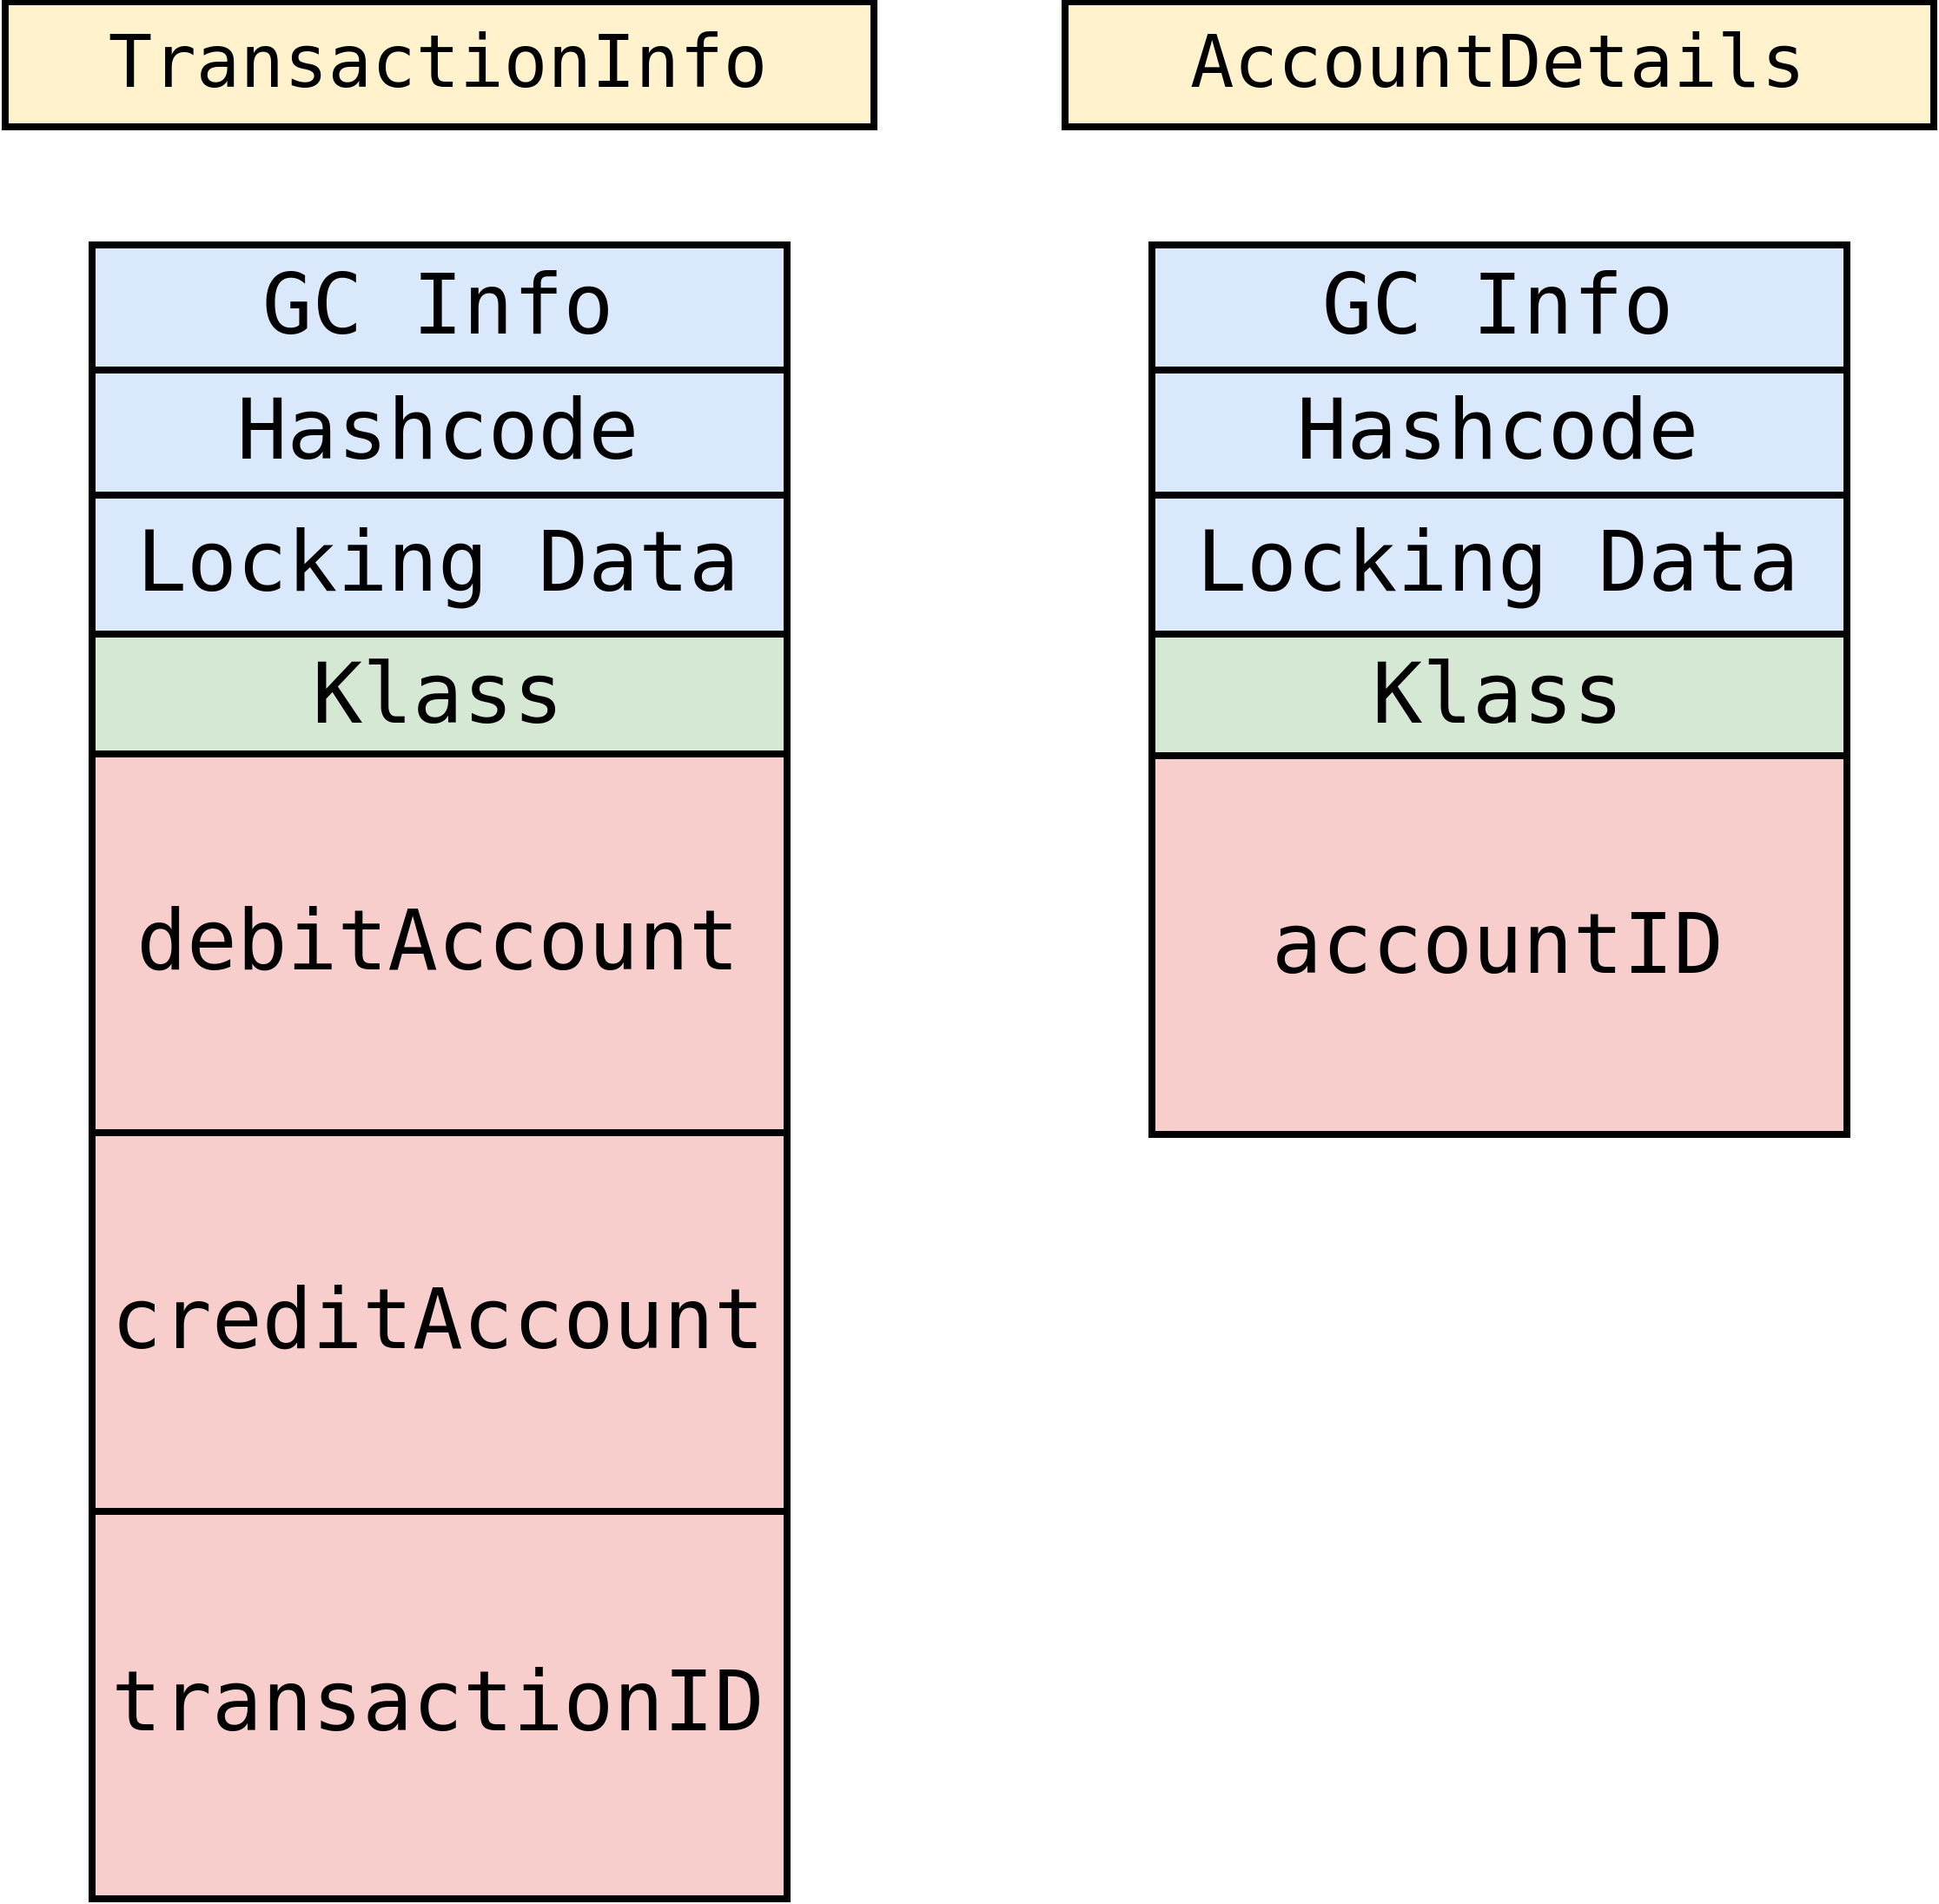
\includegraphics[scale=0.35]{images/TransactionInfo-Structure.png}
      % \caption\small{Memory Layout of TransactionInfo and AccountDetails object.}
      % \caption{Object layout of the classes.}
    \end{figure}
\end{columns}
\end{frame}

%------------------------- 3. OBJECT STRUCTURE SLIDE -----------------------%

%------------------------- 3. OBJECT STRUCTURE SLIDE -----------------------%
\begin{frame}[noframenumbering]{Object Structure}
  \begin{columns}[T,onlytextwidth] 
    \column{0.45\textwidth} 
    \begin{figure}
      \lstinputlisting[style=code]{code/TransactionInfo.java}
    \end{figure}
    \vfill
    \column{0.55\textwidth} 
    \begin{figure}
      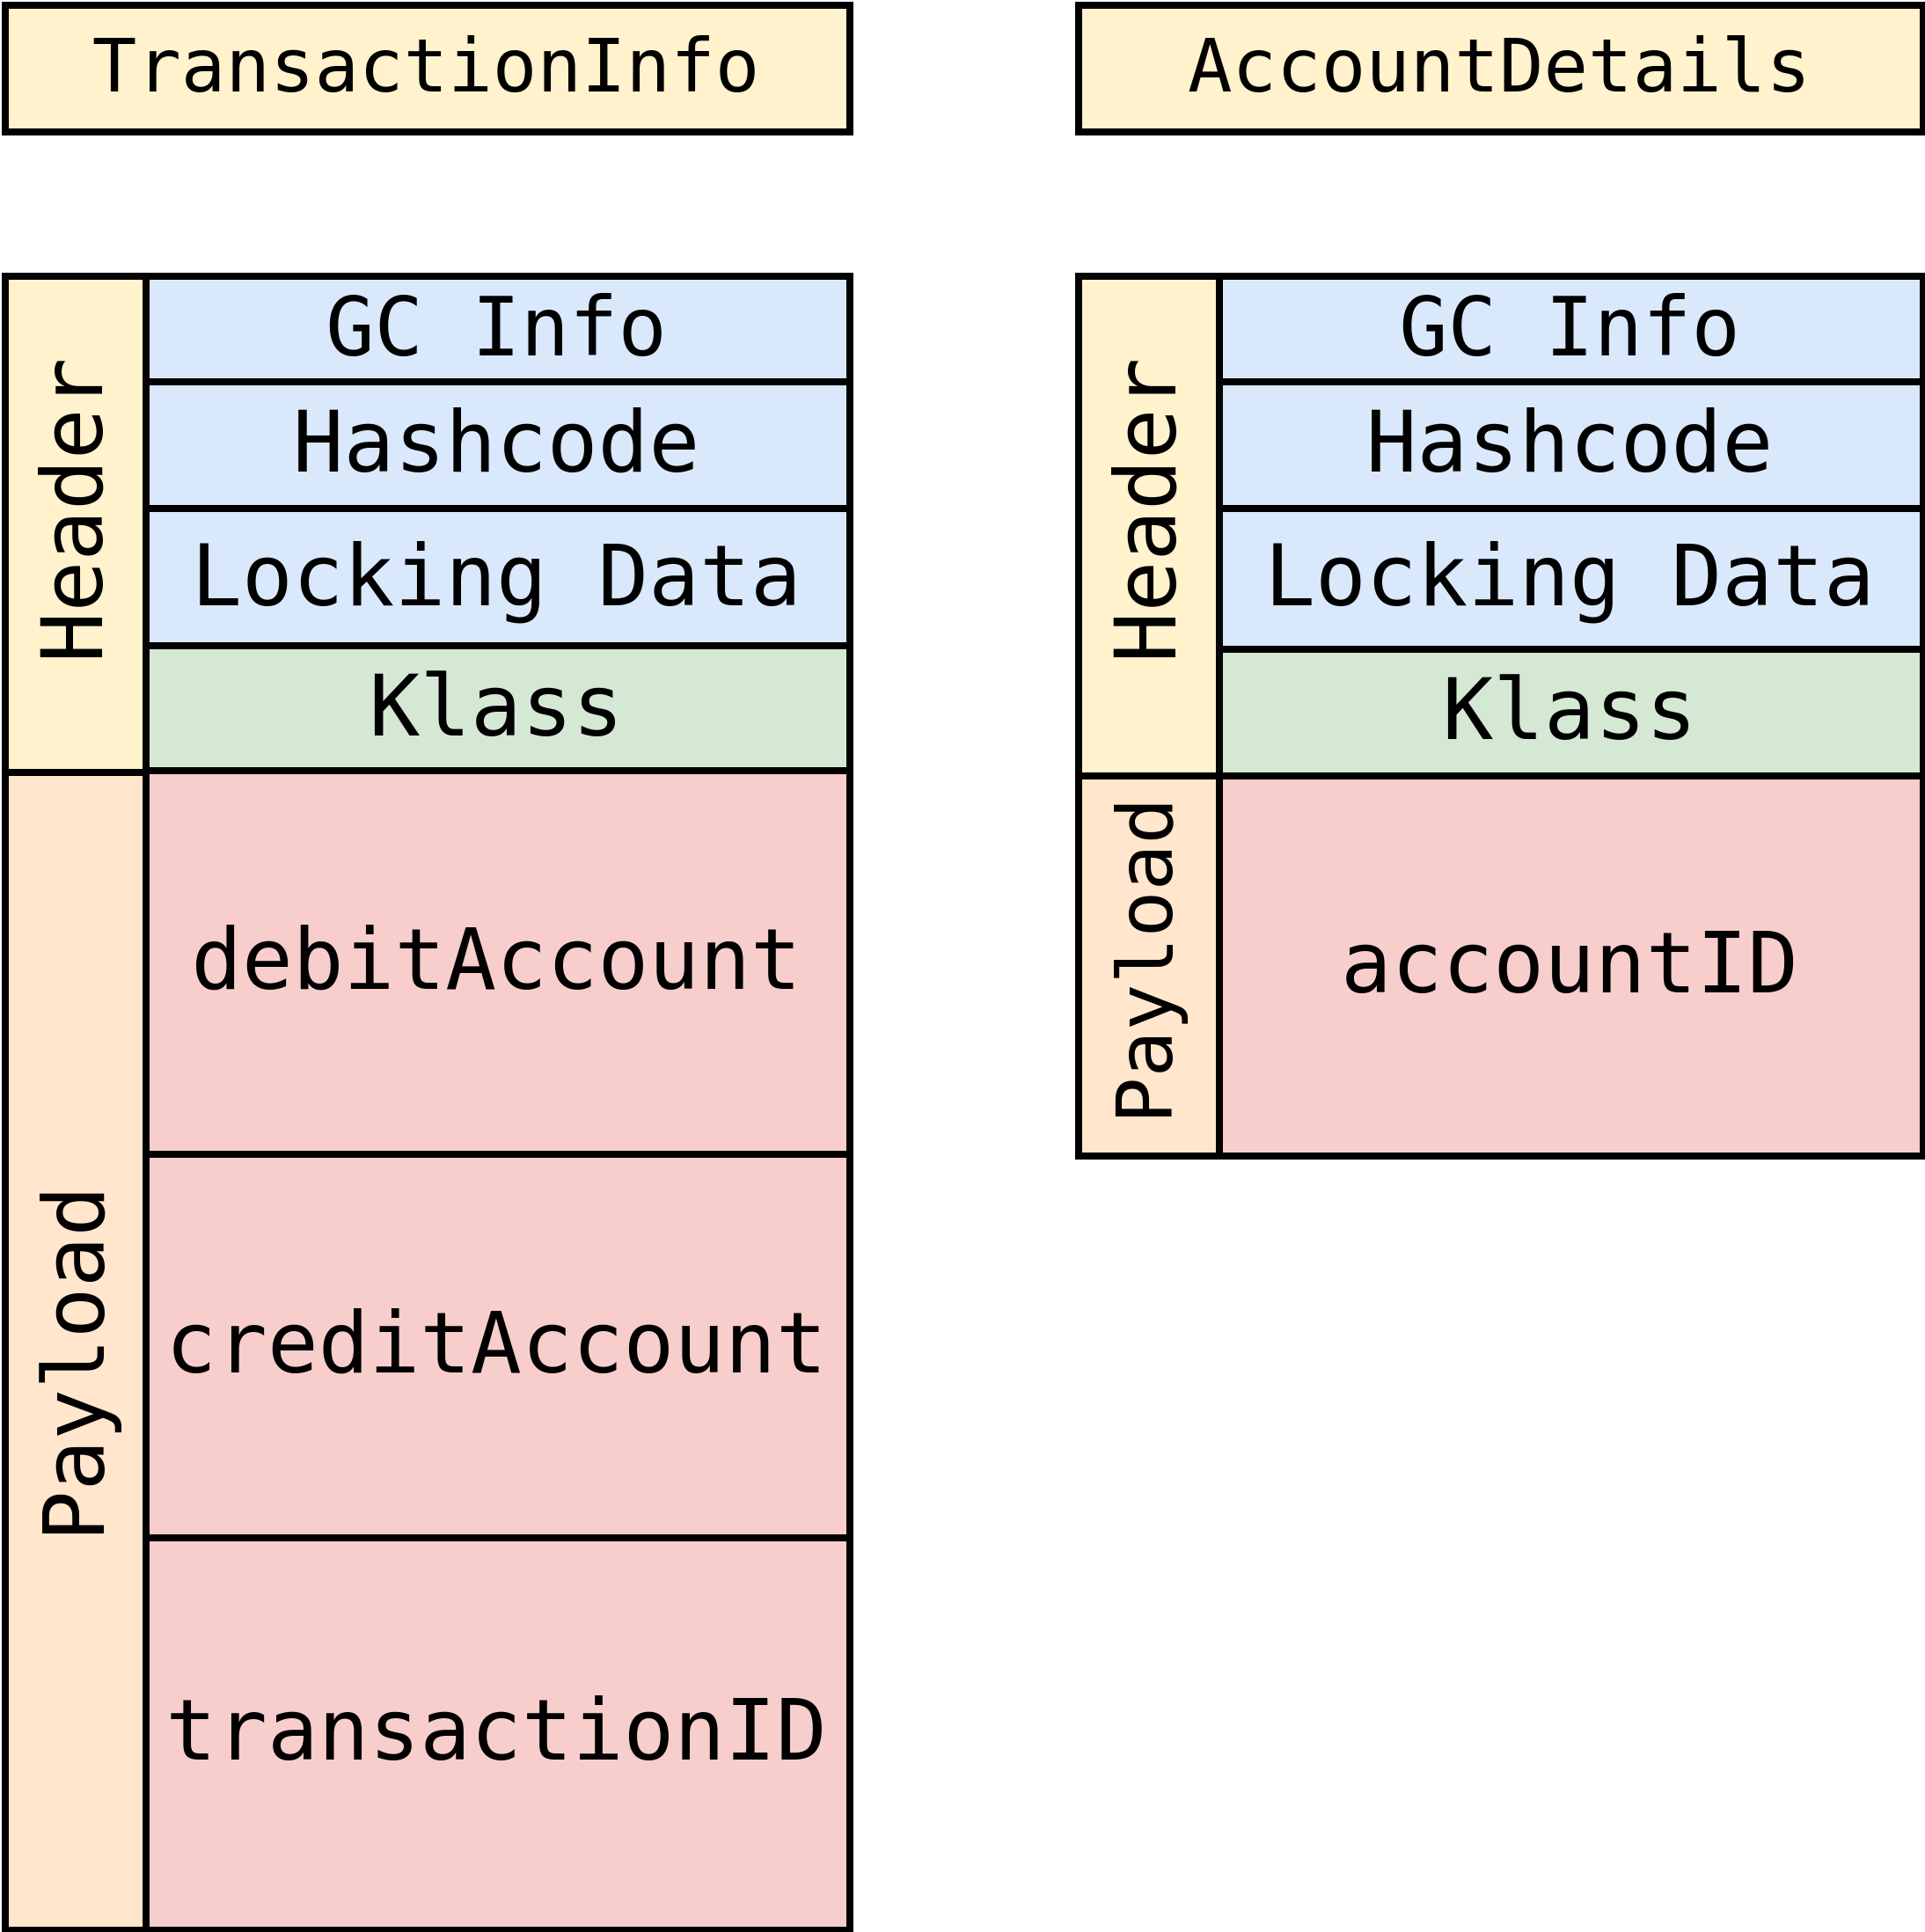
\includegraphics[scale=0.35]{images/TransactionInfo-Structure-Detailed.png}
      % \caption\small{Memory Layout of TransactionInfo and AccountDetails object.}
    \end{figure}
\end{columns}
\end{frame}

%------------------------- 3. OBJECT STRUCTURE SLIDE -----------------------%


%------------------------- 4. OVERHEADS IN OBJECT STRUCTURE SLIDE -----------------------%
\begin{frame}{Overheads}
    \begin{varblock}[13cm]{}
        \begin{itemize}
        \item Object identity serves only to support mutability.
        % \item An object’s state can be mutated but remains the same intrinsic object.
        \item Not all objects require identity.
        \item Objects that maintain identity are allocated in the heap unless optimized by the compiler.
        \item Information required to maintained identity is stored in object header.
        \item On an average 8-12 bytes are required for each object header.
        \item Compilers do not eliminate this memory overhead even when an object is immutable.
        \end{itemize}
      \end{varblock}
      \vfill
\end{frame}

%------------------------- 4. OVERHEADS IN OBJECT STRUCTURE SLIDE -----------------------%


%------------------------- 5. FIELD ACCESS SLIDE -----------------------%
\begin{frame}{Field Access}
        \begin{itemize}
        \item Memory indirections are costly.
        \item Field accesses require multiple indirection(s).
        \item Consider the statement: 
        
        \tt{int val = transactionInfo.creditAccount.accountId}
        \end{itemize}
        \vspace{0.5cm}
        \begin{figure}
          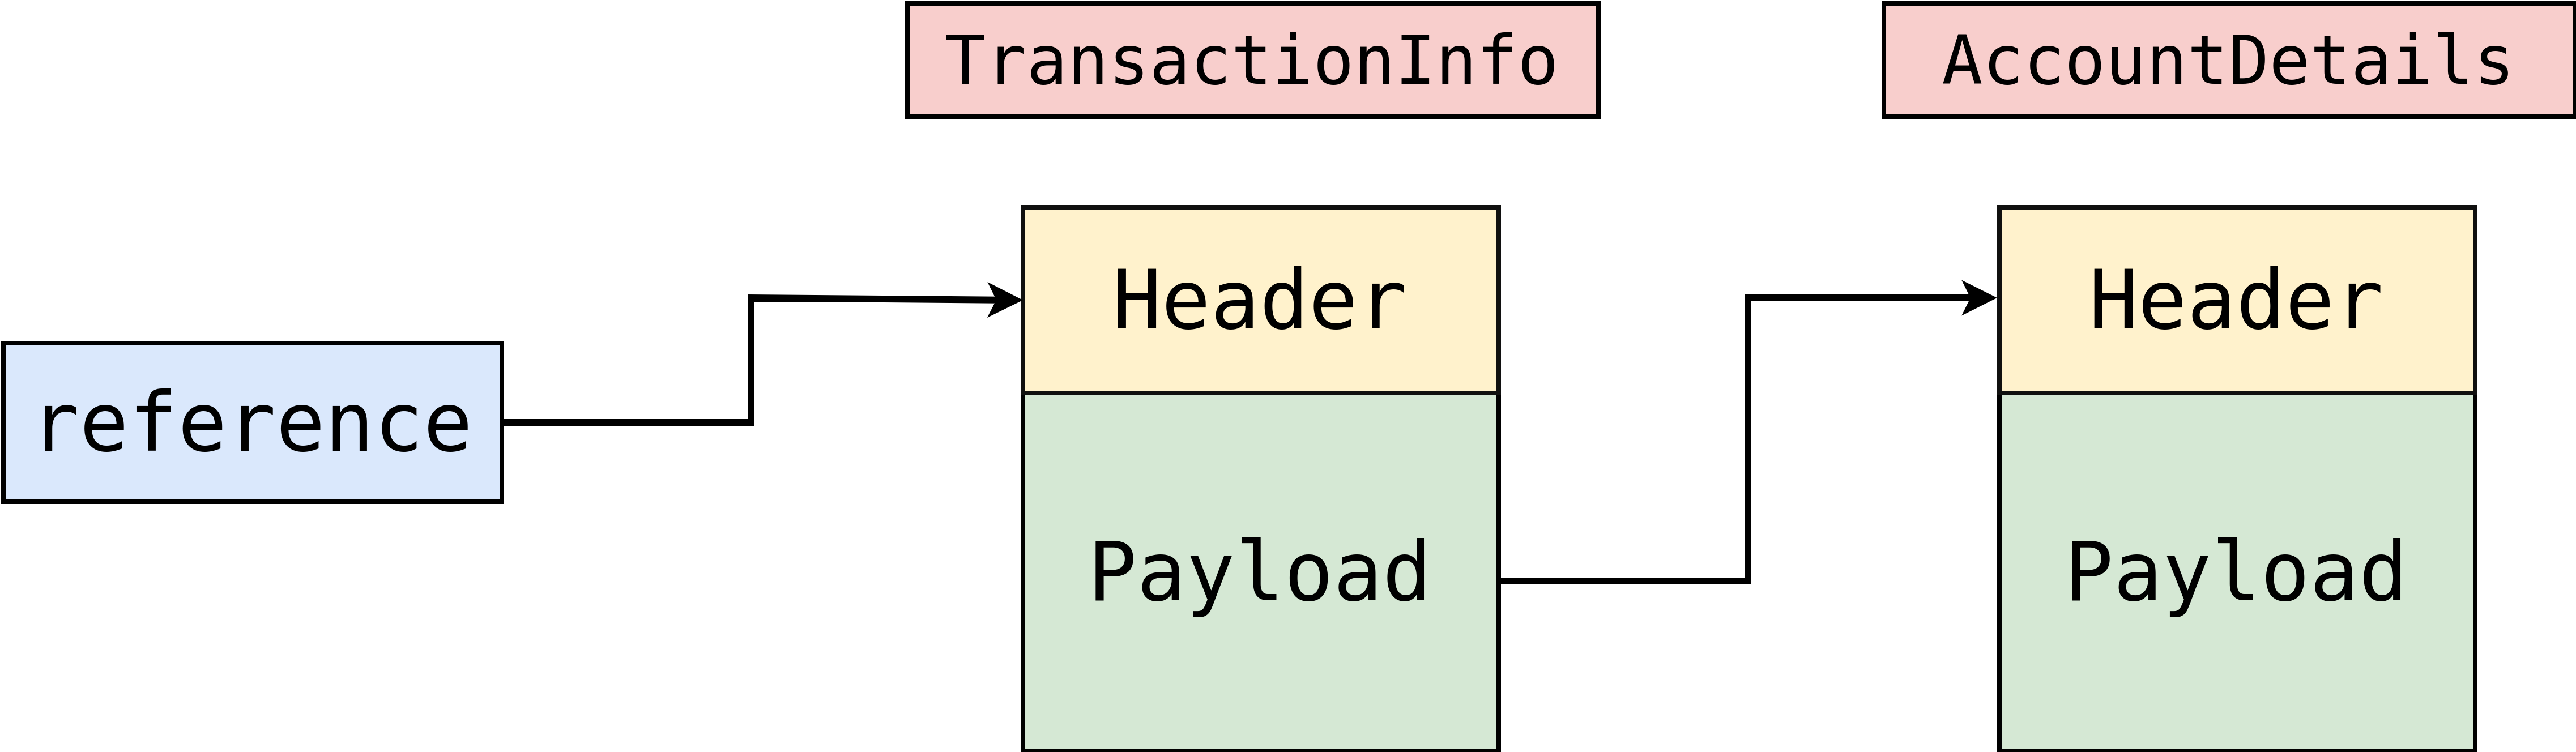
\includegraphics[scale=0.3]{images/Field_Indirections.png}
        \end{figure}
      \vfill
\end{frame}

%------------------------- 5. FIELD ACCESS SLIDE -----------------------%

%------------------------- 6. HEAP SNAPSHOT SLIDE -----------------------%
\begin{frame}{Heap Snapshot}
  \begin{itemize}
    \item Heap memory becomes a collection of data-islands.
  \end{itemize}
  \begin{figure}
    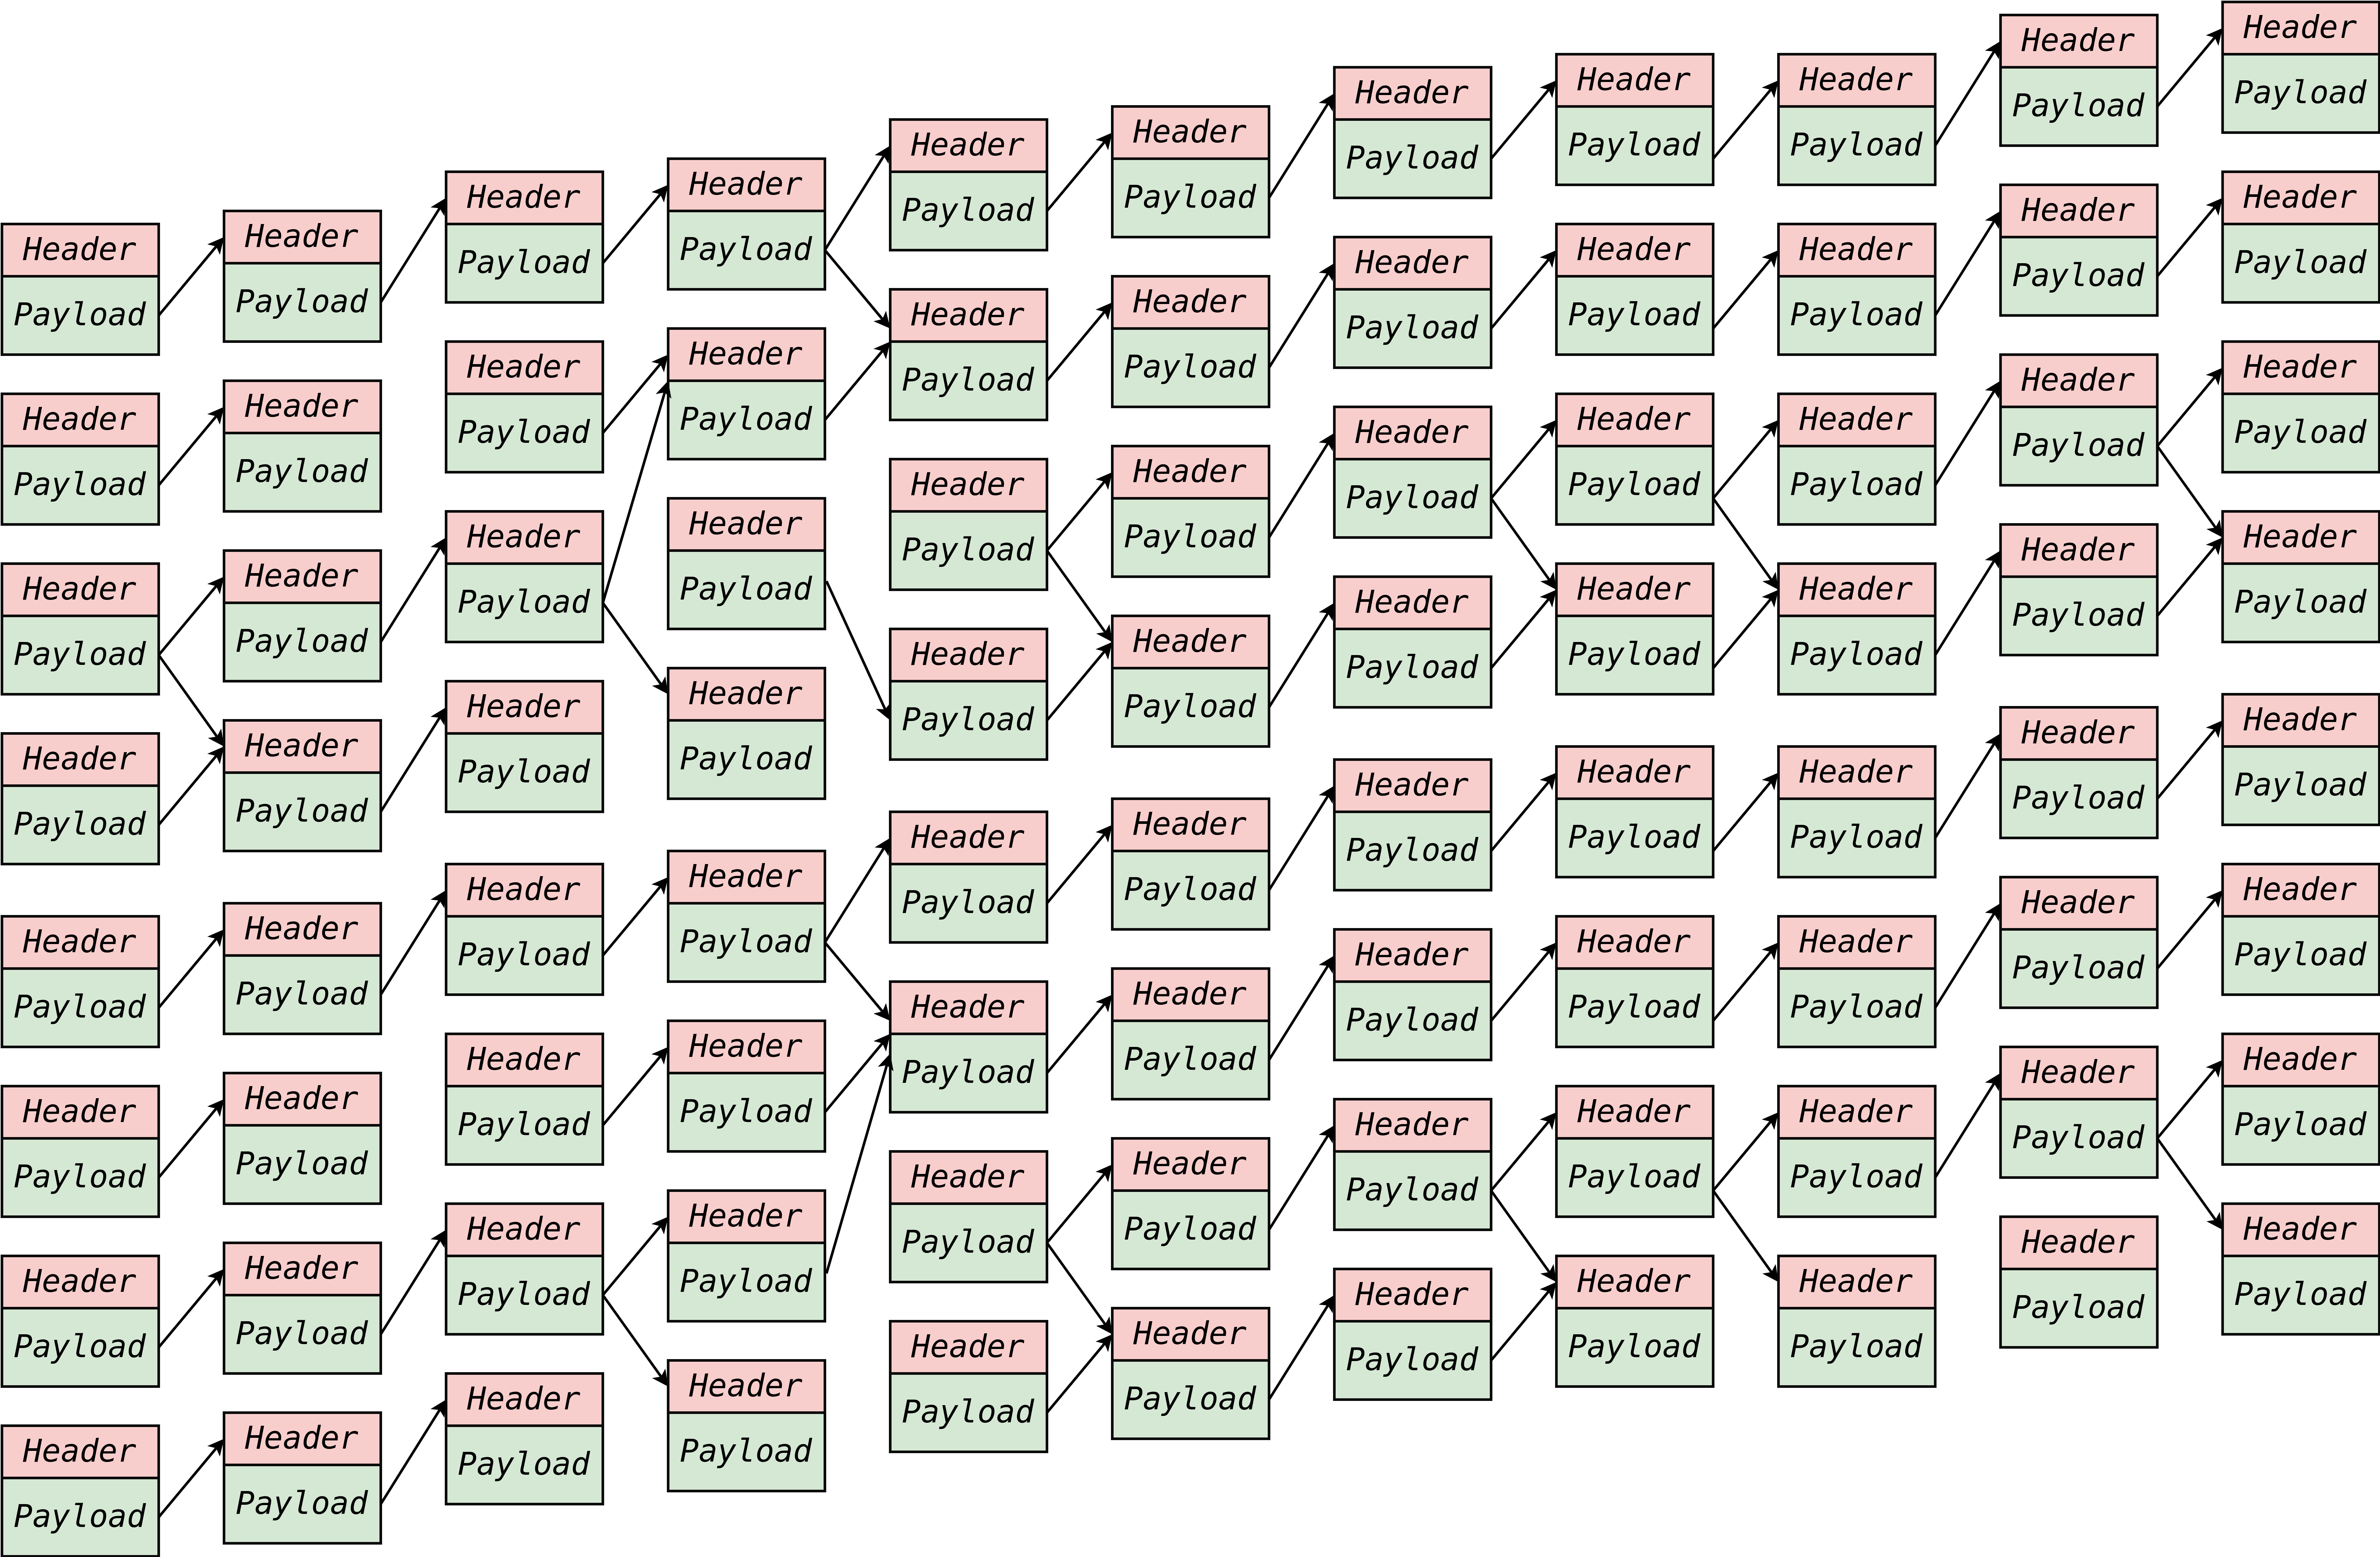
\includegraphics[scale=0.2]{images/Heap-Snapshot.png}
  \end{figure}
\vfill
\end{frame}

%------------------------- 6. HEAP SNAPSHOT SLIDE -----------------------%

%------------------------- 7. PROBLEM SUMMARY SLIDE -----------------------%
\begin{frame}{Problems?}
  \begin{varblock}[11cm]{Too many indirections!}
    \begin{itemize}
      \item Memory access is costly.
      \item Increased probablity of cache-misses.
    \end{itemize}
  \end{varblock}
  \begin{varblock}[11cm]{Too many references!}
    \begin{itemize}
      \item Increased memory footprint.
      \item More GC cycles.
    \end{itemize}
  \end{varblock}
  \begin{varblock}[11cm]{Too much memory allocated for header!}
    \begin{itemize}
      \item Redundant memory allocation.
      \item Bloated objects.
    \end{itemize}
  \end{varblock}
\end{frame}
%------------------------- 7. PROBLEM SUMMARY SLIDE -----------------------%

%------------------------- 8. OBJECT INLINING SLIDE -----------------------%
\begin{frame}{Solution}
  \begin{varblock}[13cm]{Object Inlining}
    \begin{itemize}
    \item Object Inlining is a memory layout optimization that produces a compact memory representation.
    % \item Applicable to a pair of objects ${<m,n>}$ where {\tt{m}} is a field instance accessible from {\tt{n}}.
    \item A field object when inlined is encoded directly into the object which contains it. {\tt{(Container)}}
    \item An object must possess a fixed flattenable layout in order to become inlineable.
    \item Immutable objects with primitive fields are ideal candidates.
    \end{itemize}
  \end{varblock}
\vfill
\end{frame}

%------------------------- 8. OBJECT INLINING SLIDE -----------------------%

%------------------------- 9. OBJECT INLINING DEMO SLIDE -----------------------%
\begin{frame}{Object Inlining}
  \begin{figure}
    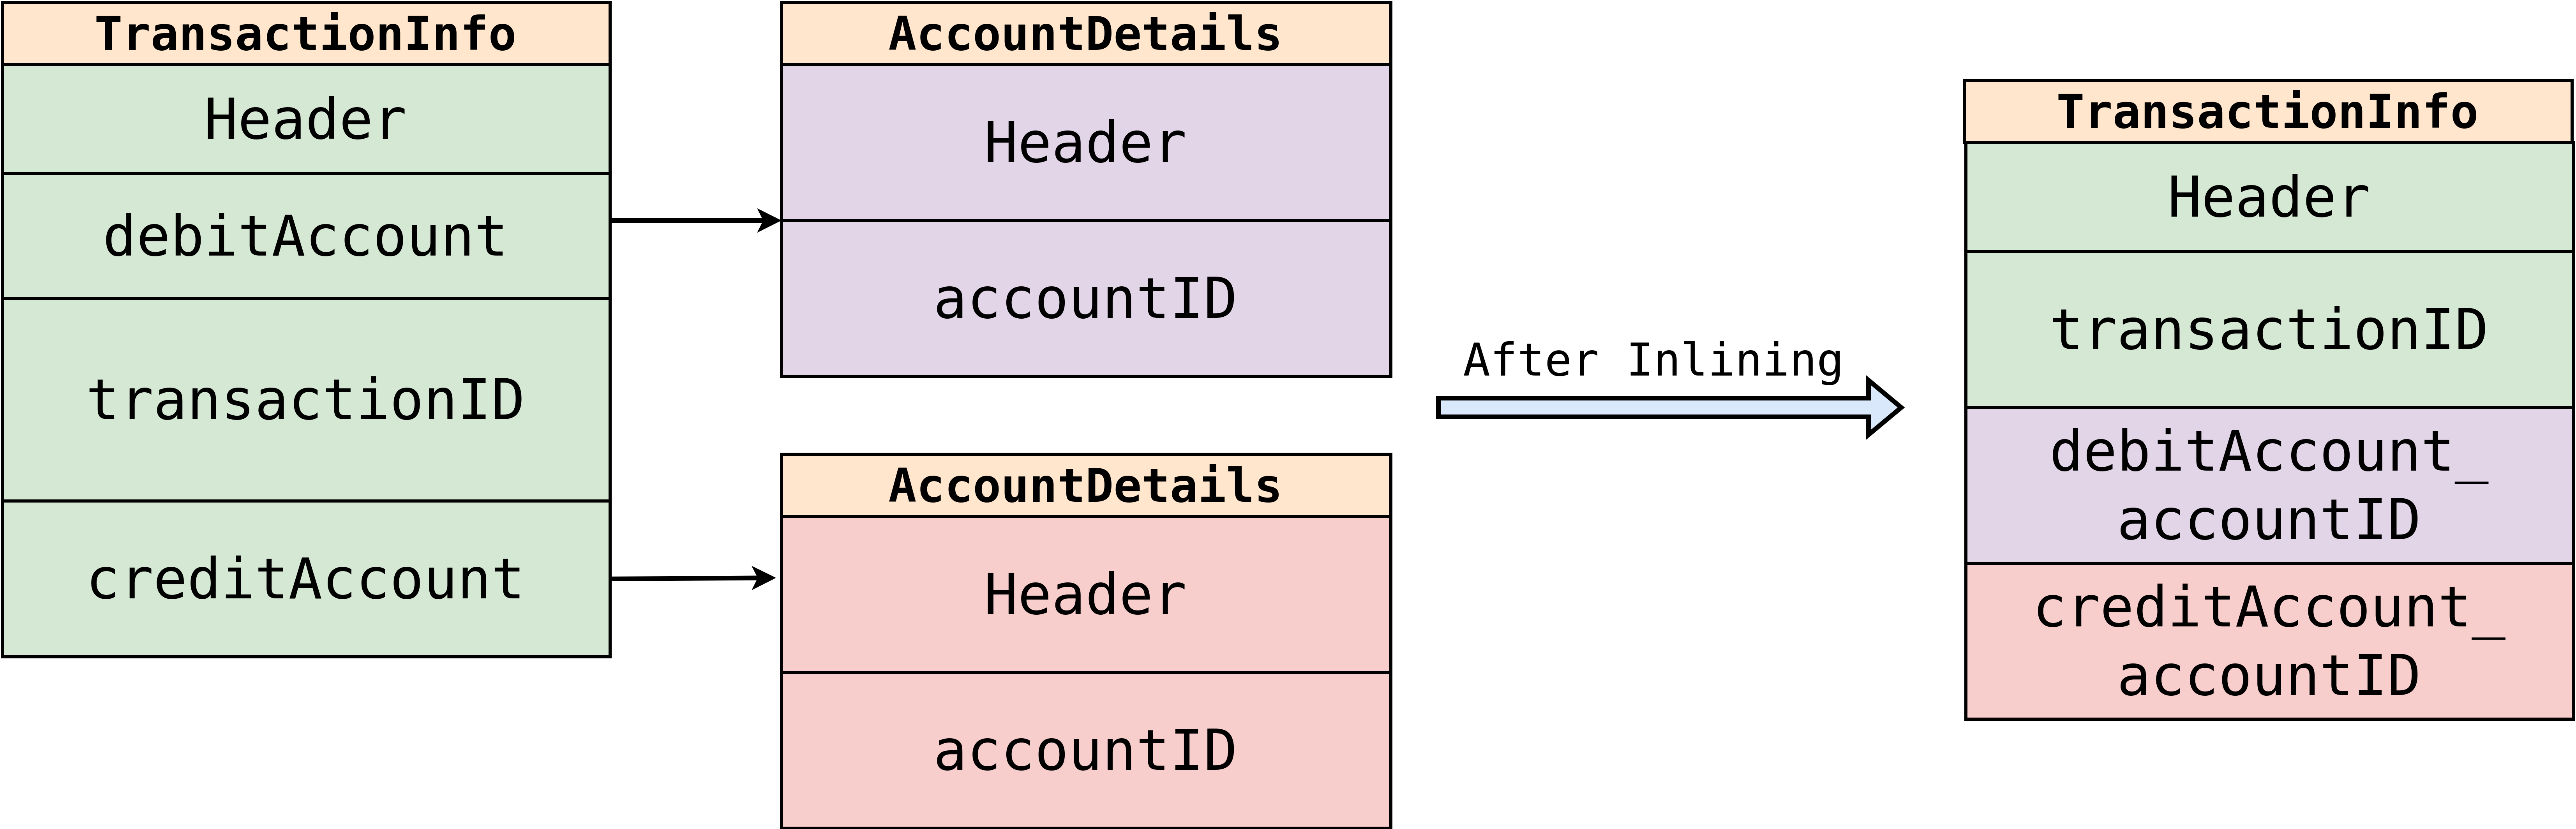
\includegraphics[scale=0.32]{images/Flattened_Transaction.png}
  \end{figure}
\end{frame}
%------------------------- 9. OBJECT INLINING DEMO SLIDE -----------------------%

%------------------------- 10. OBJECT INLINING BENEFITS AND CONSTRAINTS SLIDE -----------------------%
\begin{frame}{Object Inlining}
  \begin{varblock}[12.5cm]{Benefits}
    \begin{itemize}
    \item Fewer memory loads (indirections) for field access.
    \item Improved cache locality for field instances.
    \item Fewer memory allocations.
    \item Reduced memory footprint and GC load.
    \end{itemize}
  \end{varblock}
  \begin{varblock}[12.5cm]{Constraints for inlineability}
    \begin{itemize}
    \item Immutable - Final class, constant field values.
    \item Fixed layout - No circular dependencies in layout. 
    \item Self distinguishable - The values contained in an object should distinguish it from another instance of the same type.
    \item No header. (Loss of identity and related benefits.)
    \end{itemize}
  \end{varblock}
\end{frame}
%------------------------- 10. OBJECT INLINING BENEFITS AND CONSTRAINTS SLIDE -----------------------%

%------------------------- 11. CURRENT JVM IMPLEMEMTATION SLIDE -----------------------%
\begin{frame}{JVM Implementation{\footnotemark }}
  \begin{columns}[c] 
    \column{.42\textwidth} % Left column and width
     \begin{figure}[noindent]
\lstinputlisting[style=code]{code/Container_X.java}
\end{figure}
    \column{.47\textwidth} % Right column and width
     \begin{figure}[noindent]
  \small
\lstinputlisting[style=code]{code/ValueClass.java}
\end{figure}
\end{columns}
\begin{columns}[c] 
  \column{.42\textwidth} 
\begin{center}
  \begin{varblock}[11.5cm]{Threshold Condition Check}
    {\tt{instanceSize(InlineableField)} $\leq$ \tt{ValueFlatteningThreshold}}
  \end{varblock}
\end{center}
\end{columns}
\footnotetext[1]{Implementation inferred from Eclipse OpenJ9 VM JDK-21.}
\end{frame}
%------------------------- 11. CURRENT JVM IMPLEMEMTATION SLIDE -----------------------%

% %------------------------- 12. PERFORMANCE IMPACT SLIDE -----------------------%
% \begin{frame}{Paradox}
%   \begin{itemize}
%     \item Microbenchmark to test standard transaction operations.
%     % \item Escape analysis disabled run.
%   \end{itemize}
% \begin{columns}[c] 
%   \column{.5\textwidth} 
% \begin{center}
%   \begin{figure}
%     \includegraphics[scale=0.35]{images/Inlining-Performance.pdf}
%   \end{figure}
% \end{center}
% \column{.4\textwidth}
% \begin{varblock}[5.5cm]{}
%   \begin{itemize}
%     \item \small Experiment to measure the performance impact of object-inlining. 
%     \item \small Experiment was run by disabling dependent optimizations.
%     \item \small 2.47x slowdown observed when object inlining was enabled.
%   \end{itemize}
% \end{varblock}
% \end{columns}
% \vfill
% \vfill
% \vfill
% \vfill
% \vfill
% \end{frame}
% %------------------------- 12. PERFORMANCE IMPACT SLIDE -----------------------%

% %------------------------- 13. PERFORMANCE CONCERNS SLIDE -----------------------%
% \begin{frame}{Analysis}
%   \begin{varblock}[10.5cm]{Performance Analysis}
%     \begin{itemize}
%     \item Significantly higher instruction counts/execution.
%     \item Significantly higher CPU cycles/execution.
%     \item Higher number of memory loads. 
%     \item Lower cache miss rate.
%     \end{itemize}
%   \end{varblock}
%   \vfill
%   \vfill
%   \vfill
%   \vfill
%   \vfill
% \end{frame}
% %------------------------- 13. PERFORMANCE CONCERNS SLIDE -----------------------%

%------------------------- 15. ANTI-PATTERNS-1 SLIDE -----------------------%
\begin{frame}{Anti-Patterns: Field (Im)mutation}
  \begin{columns}[c] 
  \column{.45\textwidth} 
  \footnotesize
  \begin{algorithm}[H]
    \Fn{storeField($O_{imm}$ : Object, $F_{n}$ : Field, $P_{v}$ : Primitive)} {
      \textit{Type} $T_{imm}$ = \textit{getType($O_{imm}$)}\;
      \textit{Object} $O_{new}$ = \textit{alloca($T_{imm}$)}\;
      \ForEach{Field $F_{i}$ in $O_{new}$}{
        \uIf{$F_{i} == F_{n}$} {
          \textit{setFieldValue($O_{new}$,  $F_{i}$,  $P_{v}$)}\;
        }\uElse{
          \textit{Primitive} $P_{i}$ = \textit{getFieldValue($O_{imm}$,  $F_{i}$)}\;
          \textit{setFieldValue($O_{new}$,  $F_{i}$,  $P_{i}$)}\;
        }
      }
      return $O_{new}$\;
    }
	% \caption{Algorithm for storing an inlined field's value.}
  \end{algorithm}
  \column{.54\textwidth}
  \footnotesize
  \begin{itemize}
  \item Microbenchmark designed to compute the potential cost of mutation of inlined fields inside containers.
  \end{itemize}
  % \nobreakspace
  \begin{figure}
        \includegraphics[width=0.37\linewidth]{images/usecase1.pdf}
      \end{figure}
\end{columns}
\end{frame}
%------------------------- 15. ANTI-PATTERNS-1 SLIDE -----------------------%

%------------------------- 14. ANTI-PATTERNS-2 SLIDE -----------------------%
\begin{frame}{Anti-Patterns: Inlined-Field Load}
  % \footnotesize
  \begin{itemize}
  \item Microbenchmark designed to compute the potential benefits of inlined field access inside containers.
  \end{itemize}
  \begin{columns}[c] 
  \column{.48\textwidth}
    \begin{figure}[noindent]
      \begin{flushleft}
      \lstinputlisting[style=code,numbers=none]{code/EA.java}
      \end{flushleft}
    \end{figure}
  \column{.51\textwidth}
  % \nobreakspace
  \begin{figure}
        \includegraphics[width=0.4\linewidth]{images/usecase2.pdf}
  \end{figure}
\end{columns}
\end{frame}
%------------------------- 14. ANTI-PATTERNS-3 SLIDE -----------------------%
\begin{frame}{Anti-Patterns: Inlined-Field Load}
  \centering
  \begin{algorithm}[H]
    \Fn {getField($F_{n}$ : Field)} {
      \textit{Object} $O_{c}$ = \textit{getContainerObject($f_{n}$)}\;
      \uIf{$F_{n}$ is inlined} {
          \textit{Type} $T_{fn}$ = \textit{getType($f_{n}$)}\;
          \textit{Object} $O_{new}$ = \textit{alloca($T_{fn}$)}\;
          \ForEach{Field $F_{i}$ in $O_{new}$}{
              \textit{Field} $F_{ni}$ = \textit{getInlinedField($O_{c}$,  $F_{n}$,  $F_{i}$)}\;
              \textit{Primitive} $P_{i}$ = \textit{getFieldValue($O_{c}$,  $F_{ni}$)}\;
              \textit{storeField($O_{new}$,  $F_{i}$,  $P_{i}$)}\;
          }
          return $O_{new}$\;
      }\uElse{
          return \textit{getFieldValue($O_{c}$,  $F_{n}$)}\;
      }
  }
  \end{algorithm}
\end{frame}
%------------------------- 14. ANTI-PATTERNS-3 SLIDE -----------------------%



%------------------------- 16. ESCAPE ANALYSIS SLIDE -----------------------%
\begin{frame}{Correlation with Escape Analysis}
    \begin{columns}[T,onlytextwidth] 
      \column{0.5\textwidth} 
      \begin{itemize}
        \item Before Optimization
      \end{itemize}
      \begin{figure}[noindent]
        \begin{flushleft}
        \lstinputlisting[style=code,numbers=none]{code/BeforeEA.java}
        \end{flushleft}
      \end{figure}
      \column{0.5\textwidth} 
      \begin{itemize}
        \item After Optimization{\footnotemark[1]}
      \end{itemize}
      \begin{figure}[noindent]
        \lstinputlisting[style=code,numbers=none]{code/AfterEA.java}
      \end{figure}
    \end{columns}
    \footnotetext[1]{Assumption: The field instance does not escape.}
\end{frame}
%------------------------- 16. ESCAPE ANALYSIS SLIDE -----------------------%

% \begin{frame}{Should all inlineable fields be inlined?}
%   \begin{figure}
%     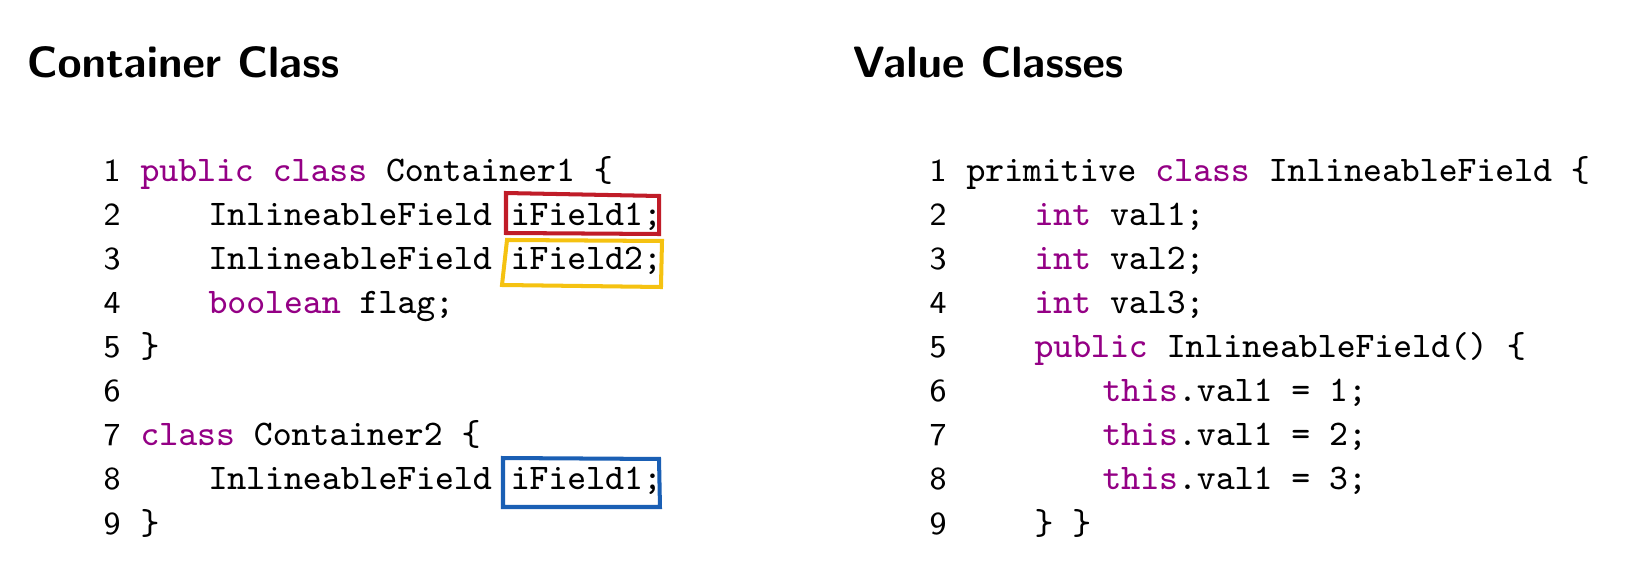
\includegraphics[scale=0.25]{images/Field_Granularity.png}
%   \end{figure}
%  \vskip 3cm
% \end{frame}

%------------------------- 17. CACHE COHERENCE SLIDE -----------------------%
\begin{frame}{Impact on Cache}
    \begin{itemize}
      \item Experiment to measure the impact of container size on the cache.
      \item Inlining has a positive impact when container size is less than 2x cache line size.
    \end{itemize}
  \begin{figure}
    \includegraphics[scale=0.5]{images/miss-rate.pdf}
  \end{figure}
\end{frame}
%------------------------- 17. CACHE COHERENCE SLIDE -----------------------%

\begin{frame}{Proposed Approach: ValFinder}
  \begin{figure}
    \includegraphics[width=0.8\linewidth]{images/Block_Digram_ValFly.pdf}
  \end{figure}
\end{frame}

\begin{frame}{Static Analyses}
  \begin{block}{Static Inlineability Analysis - SIA}
    \begin{itemize}
    \item Tool to analyze and modify source code to support value-type compliance.  
    \item Input: Source code: ({\tt .class}) and the corresponding ({\tt .java}) files.
    \item Output: Container-field metadata ({\tt .json}) along with modified source code ({\tt .java}). 
    % \item Internally Soot Optimization framework and Javaparser is used.
    \end{itemize}
  \end{block}
  \begin{figure}
    \includegraphics[width=0.6\linewidth]{images/ValFinder.pdf}
  \end{figure}
  % \begin{columns}[T,onlytextwidth] 
  %   \column{0.5\textwidth} 
  %   \begin{block}{SIA}
  %       \small
  %       \begin{itemize}
  %       \item Static analysis based tool that identifies and modifies code to support value types.  
  %       \item Input: {\em .class} files and the corresponding {\em .java} files.
  %       \item Output: Modified source code {\em .java} and container-field metadata {\em .json}.
  %       \end{itemize}
  %     \end{block}
  %   \column{0.5\textwidth} 
  %   \begin{figure}[noindent]
  %     \includegraphics[width=0.8\linewidth]{images/ValFinder.pdf}
  %   \end{figure}
  % \end{columns}
  \vfill

\end{frame}

\begin{frame}{Static Analyses}
 \begin{block}{Static Scalar Replacement Analysis - SSRA}
  \begin{itemize}
    \item Analyses to identify instructions corresponding to the identified fields that may affect program performance.
    \item Input: {\tt .class} (source code) and {\tt .json} (container-field metadata from SIA). 
    \item Output: ${\tt<Method-Signature,BCI>}$ pairs corresponding to each field. ({\tt .out}).
    \item Consists of three sub-analyses:
      \begin{itemize}
        % \small
        \item Field-Access Analysis
        % :  Identify potential local variables that could store
        references to inlined fields.
        \item Method-Summary Construction
        % : Generates a summary of methods that take in container objects as arguments.
        \item Escape Analysis
        % : Performs a static escape analysis based on the information from other analyses.
      \end{itemize}
  \end{itemize}
\end{block}
\end{frame}

\begin{frame}{Runtime Profiler}
  \centering
  \begin{block}{The two primary objectives of our runtime analyses:}
    \begin{itemize}
      \item Estimate the cost of converting each inlined field into auxilliary objects.
      \item Estimate the number of times an inlined field is beneficially accessed.
    \end{itemize}
  \end{block}
  \begin{figure}
    \includegraphics[width=0.4\linewidth]{images/Runtime-Analysis.pdf}
  \end{figure}
\end{frame}

\begin{frame}{Runtime Profiler}
  \begin{varblock}[12cm]{Runtime profiling of inlined field accesses}
    \small
    \begin{itemize}
      \item Implemented in Eclipse OpenJ9 VM.
      \item TestaRossa JIT (TRJIT) compiler is used internally for JIT compilation.
      \item TRJIT uses a tree based IL called TRIL for analysis and optimization.
      \item Debug counters is a mechanism to determine runtime execution count of individual instructions.
      \item Counters eventually get converted into machine code that collects the runtime execution count of the corresponding instruction.
      \item Our runtime profiler uses debug counters to profile instructions identified from pervious stages.
    \end{itemize}
  \end{varblock}
  % \begin{figure}
  %   \includegraphics[width=0.5\linewidth]{images/Runtime-Analysis.pdf}
  % \end{figure}
  \vfill
\end{frame}

\begin{frame}{Execution Engine}
  \begin{figure}
    \begin{block}{Field Profit Analysis}
      \begin{itemize}
        \item Runtime profiler output provides a measure of cost and benefits associated with inlining a field.
        \item Perform cost-benefit analysis for each field.
        \item Selectively identify fields which benefit from inlining.
        \item Maximum threshold size of \textbf{Container} = \textbf{2 x Cache Line Size} is verified at runtime.
        \item If the container size of {\tt Container} exceeds the threshold,
              inline fields based on FCFS approach.
      \end{itemize}
    \end{block}
  \end{figure}
\end{frame}

\begin{frame}{Execution Engine}
  \begin{figure}
    \begin{block}{Selective Inlining}
      \begin{columns}[c] 
        \column{.45\textwidth} % Left column and width
         \begin{figure}[noindent]
    \lstinputlisting[style=code]{code/Container_X.java}
    \end{figure}
        \column{.52\textwidth} % Right column and width
        \small
        \begin{itemize}
          \item Inline fields selectively rather than inlining fields of the same type across containers.
          \item {\tt iField1} can be inlined irrespective of {\tt iField2} in {\tt Container1} instance.
          \item {\tt iField3} in {\tt Container2} instance can be inlined irrespective of  or {\tt iField2} in {\tt Container1} instance.
        \end{itemize}
        % \phantom{Text}
    \end{columns}
    \vfill
    \end{block}
  \end{figure}
\end{frame}

%------------------------- 17. REAL-WORLD EXAMPLE SLIDE -----------------------%
\begin{frame}{Real-World Example}
  \begin{columns}[c] 
    \column{.5\textwidth} 
  \begin{center}
    \begin{figure}
      \includegraphics[scale=0.35]{images/Raytracer-Perf.pdf}
    \end{figure}
    \begin{itemize}
      \item \small Figure shows the performance impact of the proposed scheme in raytracer benchmark of JGF suite.
    \end{itemize}
    \end{center}
    \vfill
  \column{.4\textwidth}
  \begin{varblock}[5.5cm]{}
    \begin{itemize}
      \item \small ET: Execution time 
      \item \small C: CPU Cycles
      \item \small I: Instructions executed
      \item \small L11: L1D Cache Loads
      \item \small L12: L1D Cache Miss Rate
    \end{itemize}
  \end{varblock}
  \end{columns}
\end{frame}
%------------------------- 17. REAL-WORLD EXAMPLE SLIDE -----------------------%

%------------------------- 17. CHALLENGES AND ROAD AHEAD -----------------------%
\begin{frame}{Challenges and Road Ahead}
  \begin{block}{Challenges}
    \begin{itemize}
    \item Benchmarks with explicit inlineability do not exist for Java.
    \item Identifying inlineable fields in existing codebases is a hectic process.
    \item Manual refactoring of code almost impossible in a large codebase.
    \end{itemize}
  \end{block}
  \begin{block}{Road Ahead}
    \begin{itemize}
    \item Refactor JCL classes to support inlineability. 
    \item Prior works shows inlineable fields are mostly wrapper types in Java.
    \end{itemize}
  \end{block}
\end{frame}
%------------------------- 17. CHALLENGES AND ROAD AHEAD -----------------------%
%------------------------- 17. SUMMARY -----------------------%

\begin{frame}{Summary}
    \begin{itemize}
    \item Analyzed the current state of object-inlining optimization in Java.
    \item Identified various \textbf{access patterns} under which fields should be inlined in their
    respective containers.
    \item Built an appropriate \textbf{inlining strategy} using a static + JIT analysis technique.
    \item Developed a novel \textbf{selective} inlining scheme for the Eclipse OpenJ9 VM.
    % \item Developed a source to source transformation tool for identification of inlineable fields.
    \end{itemize}
    \phantom{\citep{spa} \citep{EAA99} \citep{CPAEA99} \citep{soot} \citep{GPO} \citep{PV}
    \citep{PYE2019} \citep{JEPP} \citep{JEPD} \citep{OpenJ9} \citep{JP}
    }
\end{frame}
%------------------------- 17. SUMMARY -----------------------%
%------------------------- 17. PUBLICATIONS -----------------------%

\begin{frame}{Publications}
  \begin{enumerate}
    \item \textbf{Arjun Harikumar} and \textbf{Manas Thakur}. “ValFinder: Finding Hidden Value-Type Classes”. 
    6th Workshop on Advances in Open Runtimes and Cloud Performance Technologies (AORCPT), part of IBM WeaveSphere, Toronto, Canada, November 16th, 2022.
    \item \textbf{Arjun H Kumar}, Hang Shao, Tobi Ajila, Vijay Sundaresan, Daryl Maier, and \textbf{Manas Thakur}.
    "Selective Value-Object Inlining using Hybrid Static and Dynamic Analysis". 
    (under review in the European Conference on Object-Oriented Programming (ECOOP), 2024)   
  \end{enumerate} 
\end{frame}
%------------------------- 17. PUBLICATIONS -----------------------%
%------------------------- 17. THESIS-ORGANIZATION -----------------------%

\begin{frame}{Thesis Organization}
  Thesis structure consists of the following six chapters:
  \begin{enumerate}
  \item \textbf{Introduction}.
  \item \textbf{Object Inlining}.
  \item \textbf{Analysis of Current Inlining Strategy}.
  \item \textbf{Hybrid Selective Inlining Strategy}.
  \item \textbf{Related Work}.
  \item \textbf{Conclusion and Future Work}.
  \end{enumerate}
\end{frame}
%------------------------- 17. THESIS-ORGANIZATION -----------------------%

%------------------------- 17. THESIS-ORGANIZATION-INTRODUCTION -----------------------%

\begin{frame}{Thesis Organiztion}
  \begin{block}{Introduction}
    \small
    This chapter briefly describes about:
    \begin{itemize}
    \item Object Oriented Languages and JIT Compilers
    \item Various design choices and current implementation of specific languages features used later in
    the thesis. 
    \item Overall JIT compilation process by using a industry standard JIT compiler as a usecase.
    \end{itemize}
  \end{block}
  \begin{block}{Object Inlining}
    \small
    This chapter describes about:
    \begin{itemize}
      \item Object Inlining optimization in depth. 
      \item Constraints imposed by modern programming languages for enabling object inlining.
    \end{itemize}
  \end{block}
\end{frame}

%------------------------- 17. THESIS-ORGANIZATION-INTRODUCTION -----------------------%

%------------------------- 17. THESIS-ORGANIZATION-Analysis of Current Inlining Strategy -----------------------%
\begin{frame}{Thesis Organiztion}
  \begin{block}{Analysis of Current Inlining Strategy}
    This chapter describes about:
    \begin{itemize}
      \item Current implementation strategy used for object inlining and dicusses
      its shortcomings and drawbacks in details.
      \item Experimentation along with the broad results performed on a
      prototype version of object inlining enabled JIT compiler for Java.
      \begin{itemize}
        \item Field-access patterns.
        \item Correlation with Escape Analysis.
        \item Correlation with Cache.
      \end{itemize}
    \end{itemize}
  \end{block}
\end{frame}
%------------------------- 17. THESIS-ORGANIZATION-Analysis of Current Inlining Strategy -----------------------%

%------------------------- 17. THESIS-ORGANIZATION-Hyrbrid Selective Inlining Strategy -----------------------%
\begin{frame}{Thesis Organiztion}
  \begin{block}{Hyrbrid Selective Inlining Strategy}
    This chapter describes about the novel inlining strategy ``ValFinder'' and the various stages in it:
    \begin{itemize}
      \item Various static analyses performed.
      \item Design and implementation of the runtime profiler.
      \item Selective inlining strategy inside the JVM.
    \end{itemize}
  \end{block}
\end{frame}
%------------------------- 17. THESIS-ORGANIZATION-Hyrbrid Selective Inlining Strategy -----------------------%

%------------------------- 17. THESIS-ORGANIZATION-Hyrbrid Selective Inlining Strategy -----------------------%
\begin{frame}{Thesis Organiztion}
  \begin{block}{Related Work}
    This chapter describes about the how other researchers have explored object inlining as well as
    immutability related optimizations in various programming paradigms.
  \end{block}
  \begin{block}{Conclusion}
    This chapter describes briefly describes the work and indicates intresting future directions along with
    various applications of the work.
  \end{block}
\end{frame}
%------------------------- 17. THESIS-ORGANIZATION-Hyrbrid Selective Inlining Strategy -----------------------%




\begin{frame}
  \Huge{\centerline{\textbf{Questions}}}
  \begin{center}
    \begin{figure}
      \includegraphics[scale=0.025]{images/questions.jpg}
    \end{figure}
  \end{center}
\end{frame}

\begin{frame}[allowframebreaks]
  \frametitle{References}
  \bibliographystyle{plainnat}
  \bibliography{biblography}
\end{frame}



\end{document}